\documentclass[a4paper,
               %boxit,
               %titlepage,   % separate title page
               %refpage      % separate references
              ]{jacow}

\ifboolexpr{bool{xetex} or bool{luatex}} % test for XeTeX/LuaTeX
 {}                                      % input encoding is utf8 by default
 {\usepackage[utf8]{inputenc}}           % switch to utf8

\usepackage{graphicx, subfigure}
\usepackage{booktabs}


\begin{document}
\title{BEAM COUPLING IMPEDANCE OF THE NEW BEAM SCREEN OF THE LHC INJECTION KICKER MAGNETS}
\author{H. Day\thanks{hugo.day@hep.manchester.ac.uk}, M.J. Barnes;  CERN, Switzerland}

\maketitle 


\begin{abstract}
The LHC injection kicker magnets (MKIs) experienced strong heating during the first operational run, identified as being caused by power loss due to wakefields induced by stored beam. Studies of the beam coupling impedance of the beam screen, a series of conductors embedded in a ceramic tube placed in the ferrite yoke to screen the ferrite from the beam, resulted in new design offering improved screening: this is predicted to reduce the heating to acceptable levels for operation with 25ns beam during run 2 of the LHC. However higher beam intensities proposed for HL-LHC operation are predicted to again cause strong heating to occur. Further studies have been carried out to reduce the beam induced power loss by optimising the beam screen design, some key results and findings of which are presented here.
\end{abstract}

\section{Introduction}

The injection kicker magnets (MKIs) are fast pulsed transmission line kicker magnets, which have a ceramic tube inserted into the ferrite yoke: this supports a number of screen conductors, designed to provide a good conducting path for the image currents of the circulating beam. One end of the screen is directly connected to the beam pipe whilst the other is capactively coupled to the beam pipe in order to preserve the fast field rise time of the magnet. Beam-induced heating due to high stored beam current lead to high temperatures being observed in devices in the LHC, including the MKIs \cite{mki-heating}. In the MKI this lead to problems as the temperature of the ferrite yoke rises above it's Curie temperature necessitating 2-3 hours waiting time between fills. Substantial work has been done reduce the power deposited by reducing the beam coupling impedance of the device - a revised beam screen was implemented on all magnets during long shutdown 1 (LS1) which is predicted to reduce the power loss to a degree where excessive heating will not be a problem with nominal LHC beam parameters [cite LHC impedance 2014]. 

The planned high luminousity upgrade of the LHC (called HL-LHC) will involve a doubling of the beam current in the LHC under current nominal parameters [cite] - this is predicted to lead to again a four fold increase in the power loss to all devices in the LHC unless counter-measures are taken. To this end further improvements to the beam screen have been studied in order to reduce the power loss into the magnet whilst continuing to ensure good high voltage (HV) performance during pulsing and good field quality for operation.


into the   \cite{mki-heatingTemp}
Building on this success a new design has been proposed to satisfy competing needs of low rates of electrical breakdown, during magnet pulsing, and a low beam coupling impedance to reduce the power lost into the structure by wakefields; in addition to meeting strict requirements for magnet operation for field rise time and flat top ripple \cite{mkiUpgrade}. 

\begin{figure}
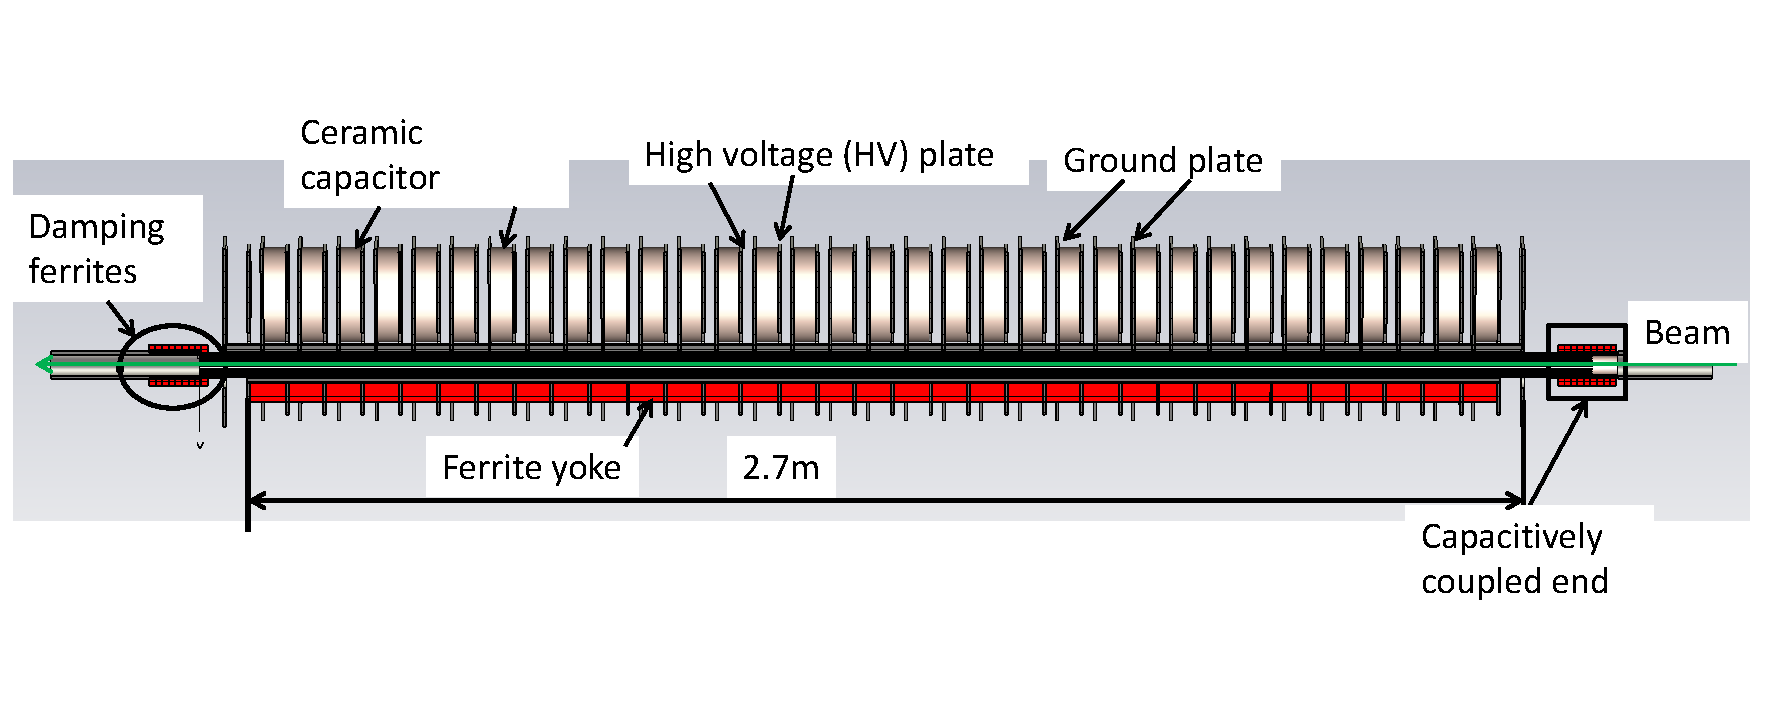
\includegraphics[width=0.5\textwidth]{MKICrossSectionYZ.pdf}
\caption{Structure of the injection kicker magnets.}
\label{fig:mkiStruct}
\end{figure}

\section{Changes to Beam Screen Design}



\begin{figure}
\begin{center}
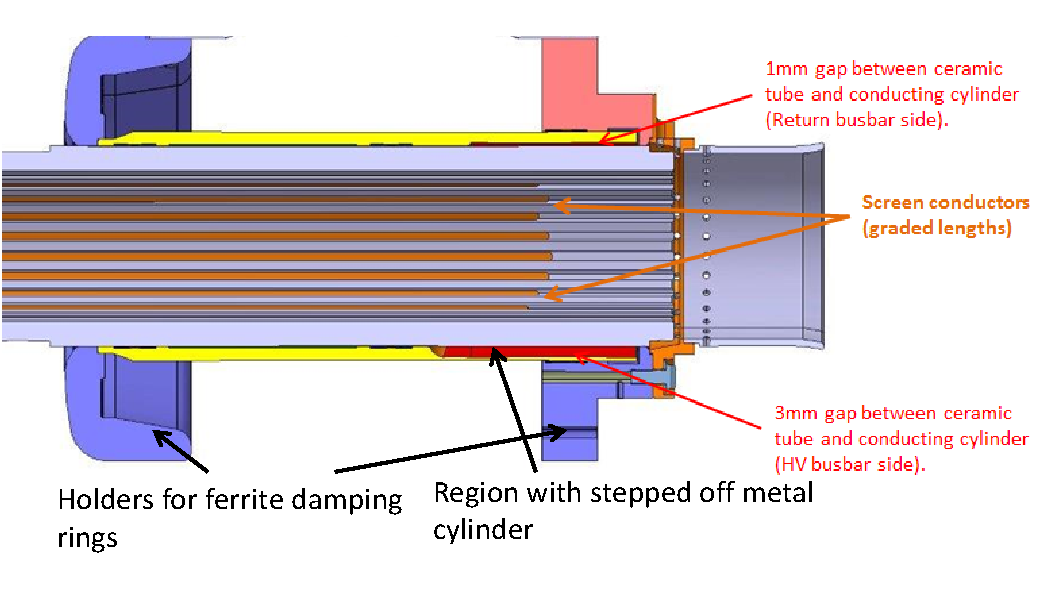
\includegraphics[width=0.5\textwidth]{beamScreenCrossSectionLabelled.pdf}
\caption{Cross section of the new beam screen design}
\label{fig:beamScreenCross}
\end{center}
\end{figure}



\section{Impedance Measurements}



\begin{figure}
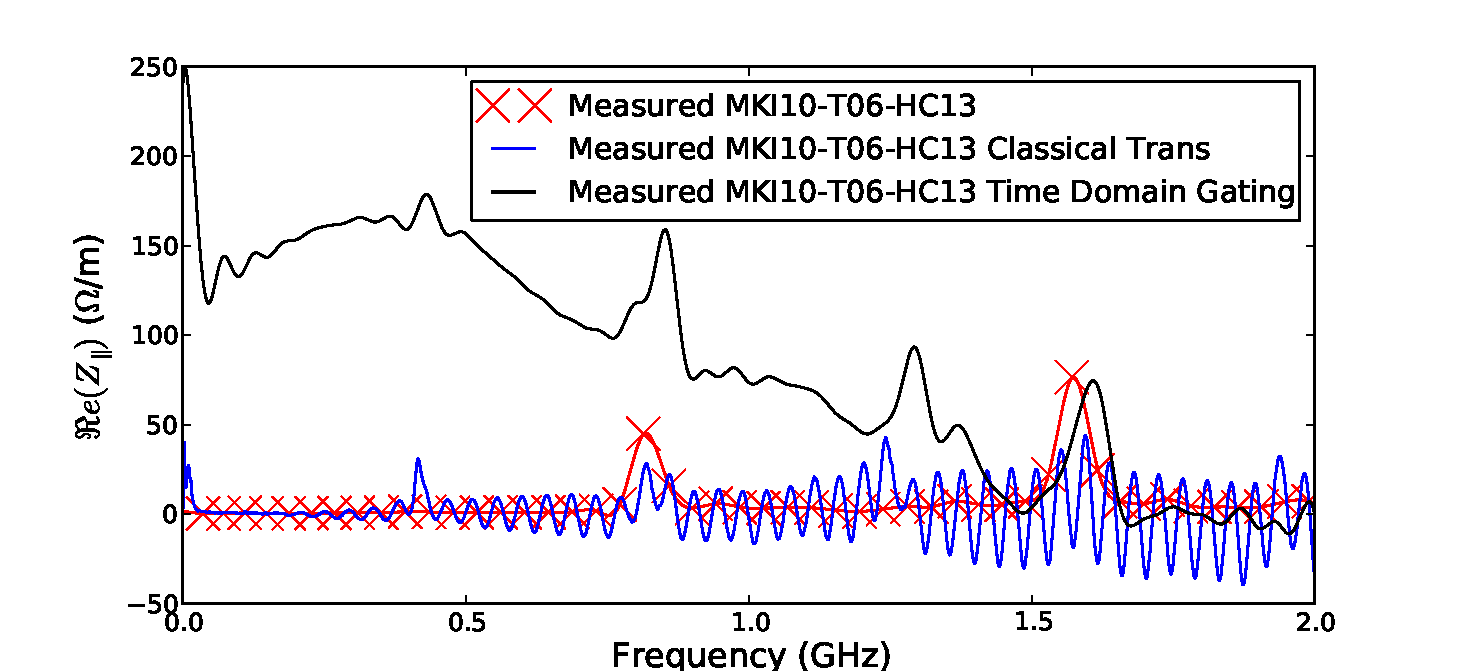
\includegraphics[width=0.45\textwidth]{compMeasurementGating.pdf}
\caption{The beam coupling impedance measurements for a magnet using either time domain gating only, or a matched resistor network in comparison to resonant coaxial wire measurements.}
\label{fig:measComp}
\end{figure}

\section{Power Loss}



\begin{equation}
P_{loss} = 2 \left( f_{0} e M  N_{b}\right)^{2} \displaystyle\sum\limits_{n = -\infty}^{\infty}  \left| \lambda \left( p M \omega_{0} \right)  \right|^{2} \Re{}e \left[ Z_{\parallel} \left( p M \omega_{0} \right) \right]
\label{eqn:powLoss}
\end{equation}


\begin{table}
\caption{Beam Parameters for different LHC operational modes}
\label{tab:beamPara}
\begin{center}
\begin{tabular}{c | c | c | c | c}
Mode & $\tau_{sep}$ (ns) & $N_{b}$ ($10^{11}$) & $ M $ & $t_{b}$ (ns) \\ \hline 
Pre-LS1 & 50 & 1.6 & $ 1380 $ & 1.2 \\ \hline 
Post-LS1 & 25 & 1.15 & 2808 & 1.0 \\ \hline 
HL-LHC, 50ns & 50 & 3.5 & 1380 & 1.0 \\ \hline 
HL-LHC, 25ns & 25 & 2.2 & 2808 & 1.0 \\ 
\end{tabular}
\end{center}
\end{table}

\begin{table}
\caption{Power Loss for different beam screen arrangements with different beam parameters (see Tab.~\ref{tab:beamPara}) in W/m.}
\label{tab:powLoss}
\begin{center}
\begin{tabular}{c | c | c}
Mode & 24 screen cond. & 15 screen cond. \\ \hline 
Pre-LS1 & 20-35 & 68 \\ \hline 
Post-LS1 & 34-52 & 117 \\ \hline 
HL-LHC, 50ns & 151-240 & 538  \\ \hline 
HL-LHC, 25ns & 125-191 & 432  \\ 
\end{tabular}
\end{center}
\end{table}

\section{Future Plans}


\section{Summary}




\begin{thebibliography}{9}

\bibitem{mki-heating}
M.J. Barnes \emph{et al}., \emph{"Analysis of Measured Ferrite Heating of the LHC Injection Kickers and Proposals for Future Reduction of Temperature"}, IPAC'12, New Orleans, USA, 2012, TUPPR090.

\bibitem{mki-heatingTemp}
M.J. Barnes \emph{et al}., \emph{"Beam Induced Ferrite Heating of the LHC Injection Kickers and Proposals for Improved Cooling"}, IPAC'13, Shanghai, China, MOPWA031.

\bibitem{mkiUpgrade}
M.J. Barnes \emph{et al}., \emph{Upgrade of the LHC Injection Kicker Magnets}, IPAC'13, Shanghai, China, MOPWA030

\bibitem{mki-ElecBreakdown}
M.J. Barnes \emph{et al}., \emph{"Reduction of Surface Flashover of the Beam Screen of the LHC Injection Kickers"}, IPAC'13, Shanghai, China, MOPWA031.

\bibitem{DayThesis}
PhD Thesis, H. Day, 2013.

\bibitem{mkiCoolling}
M. Barnes \emph{et al}., \emph{"Cooling of the LHC Injection Kicker Magnet Ferrite Yoke: Measurements and Future Proposals"}, MOPME075, these proceedings.

\bibitem{cst-cite}
\texttt{http://www.cst.com}.

\end{thebibliography}
\end{document}

